% ============================================================
% TaxiPulse — Zeroth Review Presentation (Beamer)
% 23AID302 - Big Data Analytics
% Compile on Overleaf (pdfLaTeX) or any full TeX distribution
% >>> Replace the team member names / reg. numbers on the title slide <<<
% ============================================================
\documentclass[aspectratio=169]{beamer}

\usetheme{Madrid}
\usecolortheme{default}

% Accent color (deep taxi-yellow / amber on dark blue base)
\definecolor{pulseblue}{RGB}{20,60,110}
\definecolor{pulseyellow}{RGB}{245,180,0}
\setbeamercolor{palette primary}{bg=pulseblue,fg=white}
\setbeamercolor{palette secondary}{bg=pulseblue!80,fg=white}
\setbeamercolor{palette tertiary}{bg=pulseblue!60,fg=white}
\setbeamercolor{structure}{fg=pulseblue}
\setbeamercolor{title}{bg=pulseblue,fg=white}
\setbeamercolor{frametitle}{bg=pulseblue,fg=white}

\usepackage{tikz}
\usetikzlibrary{arrows.meta,positioning}
\usepackage{booktabs}
\usepackage{array}

\setbeamertemplate{navigation symbols}{}
\setbeamertemplate{itemize item}{\color{pulseblue}$\blacktriangleright$}
\setbeamertemplate{itemize subitem}{\color{pulseyellow}$\bullet$}

% ------------------------------------------------------------
\title[TaxiPulse]{TaxiPulse: Real-Time Taxi Demand Forecasting\\ with Fare and ETA Prediction}
\subtitle{Zeroth Review}
\author[Team TaxiPulse]{%
  \textbf{Group-6}\\[4pt]
  \begin{tabular}{@{}l c l@{}}
    Pranav Kumar Reddy & -- & CB.AI.U4AID24069 \\
    Tharun Kumar Reddy & -- & CB.AI.U4AID24033 \\
    Rajdeep K          & -- & CB.AI.U4AID24022 \\
    M Hemanth Reddy    & -- & CB.AI.U4AID24066 \\
  \end{tabular}}
\institute[]{Department of Artificial Intelligence and Data Science\\[2pt]
  \textbf{23AID302 -- Big Data Analytics}}
\date{Academic Year 2026--27}

\begin{document}

% ---------------- 1. TITLE SLIDE ----------------
\begin{frame}
  \titlepage
\end{frame}

% ---------------- 2. INTRODUCTION TO THE PROBLEM DOMAIN ----------------
\begin{frame}{Introduction to the Problem Domain}
  \textbf{Domain: Big Data Analytics in Urban Transportation (Smart Mobility)}
  \begin{itemize}
    \item Urban transportation generates massive continuous data: every taxi /
          ride-hailing trip produces a record (pickup, drop, time, distance, fare).
    \item A single city like New York generates \textbf{100+ million trip records
          per year} --- far beyond the capacity of traditional tools (Excel, pandas, RDBMS).
    \item Ride-hailing platforms (Uber, Ola, Lyft) depend on analytics over this
          data for driver allocation, upfront pricing, and surge management.
  \end{itemize}
  \vspace{4pt}
  \textbf{Why this domain matters}
  \begin{itemize}
    \item Mismatch between taxi supply and demand $\Rightarrow$ idle drivers in
          quiet zones, long passenger waits in busy zones, lost revenue.
    \item Cities need demand insights for transport planning and policy.
    \item The domain naturally exhibits all 4 V's of Big Data ---
          \textbf{Volume, Velocity, Variety, Veracity} --- making it an ideal
          candidate for distributed analytics with Hadoop and Spark.
  \end{itemize}
\end{frame}

% ---------------- 3. PROBLEM STATEMENT ----------------
\begin{frame}{Problem Statement}
  \begin{block}{Problem Statement}
    Taxi fleets and ride-hailing platforms cannot efficiently position drivers or
    quote reliable prices because taxi demand fluctuates sharply with time,
    location, and weather. Existing small-scale analyses cannot process
    city-scale trip data (20+ GB, hundreds of millions of records) or react to
    live conditions. There is a need for a \textbf{scalable big data pipeline}
    that processes massive historical trip data \textbf{and} a live trip stream
    to forecast \textbf{zone-wise taxi demand for the next hour} and predict the
    \textbf{fare and ETA} of individual trips in real time.
  \end{block}
  \vspace{4pt}
  \textbf{The 4 V's in our problem}
  \begin{itemize}
    \item \textbf{Volume:} 20--50 GB of NYC trip records (200M+ trips, 2022--2024).
    \item \textbf{Velocity:} live trip stream processed with Spark Structured Streaming.
    \item \textbf{Variety:} structured trip records (Parquet/CSV) + semi-structured
          weather and zone data (JSON/GeoJSON).
    \item \textbf{Veracity:} noisy records --- negative fares, zero-passenger trips,
          invalid GPS coordinates, missing values.
  \end{itemize}
\end{frame}

% ---------------- 4. EXISTING SYSTEM / LITERATURE REVIEW ----------------
\begin{frame}{Existing System / Literature Review}
  \scriptsize
  \begin{tabular}{p{0.30\textwidth} p{0.33\textwidth} p{0.28\textwidth}}
    \toprule
    \textbf{Work} & \textbf{Contribution} & \textbf{Limitation / Gap} \\
    \midrule
    \emph{Math.\ Biosciences \& Eng.} (2024) --- ST-enhanced GCN &
    Graph convolutional network with external spatio-temporal factors for
    ride-hailing demand prediction &
    Demand only; GPU-centric deep model; ignores fare/ETA; not real time \\
    \addlinespace
    Guo et al., \emph{Applied Soft Computing} (2025) &
    Multi-gated deep graph network with attention mechanisms for taxi
    demand prediction &
    Demand only; offline training/evaluation; no distributed big data pipeline \\
    \addlinespace
    \emph{arXiv:2407.01262} (2024) --- Deep + tree fusion for ETA &
    Complementary fusion of deep networks and tree models for ETA
    prediction &
    ETA only; no demand or fare modelling; no streaming deployment \\
    \addlinespace
    \emph{Springer LNNS} (2025) --- Trip duration model comparison &
    Compares Decision Tree, Random Forest, LightGBM and Gradient Boosting for
    NYC taxi trip duration prediction &
    Single-machine study; duration only; no live prediction or dashboard \\
    \addlinespace
    \emph{Int.\ J.\ Info.\ Eng.\ \& Science} (2025) &
    Scalable fare prediction on NYC taxi trips using Spark and distributed ML &
    Fare only; no demand forecasting, no streaming, no visualization \\
    \bottomrule
  \end{tabular}
\end{frame}

\begin{frame}{Research Gaps Identified}
  \begin{itemize}
    \item \textbf{Fragmented solutions:} prior works solve demand \emph{or} fare
          \emph{or} ETA in isolation --- no unified system covers all three.
    \item \textbf{Scale gap:} most studies sample the data down to what fits on
          one machine instead of processing the full corpus distributively.
    \item \textbf{No real-time layer:} models are trained and evaluated offline;
          few works consume a live stream and update predictions continuously.
    \item \textbf{Weather ignored:} demand is highly weather-sensitive, yet many
          models exclude external context data.
    \item \textbf{No end-user visualization:} results stay in papers/notebooks;
          rarely delivered as a live decision-support dashboard.
  \end{itemize}
  \vspace{4pt}
  \begin{alertblock}{Our opportunity}
    Combine all three predictions in one \textbf{distributed batch + streaming}
    pipeline on the full 20+ GB dataset, enriched with weather, delivered
    through a live dashboard.
  \end{alertblock}
\end{frame}

% ---------------- 5. PROPOSED SYSTEM ----------------
\begin{frame}{Proposed System --- TaxiPulse}
  \textbf{Idea in one line:} learn demand/fare/ETA patterns from 200M+ historical
  trips (batch), then apply them to a live trip stream to predict what happens
  \emph{next} (real time).
  \vspace{6pt}
  \begin{center}
  \resizebox{0.95\textwidth}{!}{%
  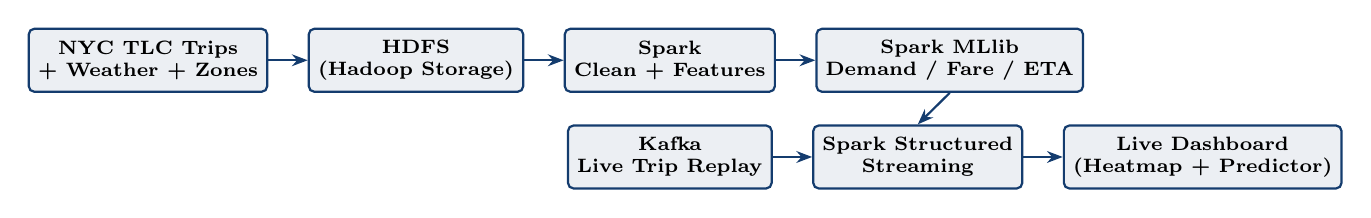
\begin{tikzpicture}[
      node distance=4mm and 5mm,
      box/.style={draw=pulseblue, thick, rounded corners=2pt, align=center,
                  font=\scriptsize\bfseries, fill=pulseblue!8,
                  minimum height=8mm, minimum width=21mm},
      arr/.style={-{Stealth[length=2mm]}, thick, pulseblue}]
    \node[box] (data) {NYC TLC Trips\\ + Weather + Zones};
    \node[box, right=of data] (hdfs) {HDFS\\ (Hadoop Storage)};
    \node[box, right=of hdfs] (spark) {Spark\\ Clean + Features};
    \node[box, right=of spark] (ml) {Spark MLlib\\ Demand / Fare / ETA};
    \node[box, below=of spark] (kafka) {Kafka\\ Live Trip Replay};
    \node[box, right=of kafka] (stream) {Spark Structured\\ Streaming};
    \node[box, right=of stream] (dash) {Live Dashboard\\ (Heatmap + Predictor)};
    \draw[arr] (data) -- (hdfs);
    \draw[arr] (hdfs) -- (spark);
    \draw[arr] (spark) -- (ml);
    \draw[arr] (kafka) -- (stream);
    \draw[arr] (ml.south) -- (stream.north);
    \draw[arr] (stream) -- (dash);
  \end{tikzpicture}}
  \end{center}
  \vspace{2pt}
  \textbf{Improvements over existing systems:} full-scale distributed processing
  (no sampling); batch \textbf{and} streaming in one pipeline; weather-aware models.
\end{frame}

\begin{frame}{Proposed System --- Novelty}
  \textbf{What is new in TaxiPulse}
  \begin{itemize}
    \item \textbf{Unified triple prediction:} one pipeline, one feature store,
          three outputs --- zone-wise demand (next hour), trip fare, and ETA.
    \item \textbf{Hybrid batch + streaming design:} models trained on the full
          historical corpus are applied to a live Kafka stream, and live demand
          pace is compared against forecasts to raise \textbf{anomaly alerts}
          (e.g., event surge, transit outage).
    \item \textbf{Context-aware forecasting:} weather (rain/temperature) and
          calendar signals (holiday, weekend) fused with trip history.
    \item \textbf{Zone behaviour discovery:} K-Means clustering automatically
          labels zones as airport / office / nightlife types from their
          24-hour demand signature.
    \item \textbf{Decision-support delivery:} live heatmap for drivers,
          fare--ETA widget for passengers, monitoring panel for operators.
  \end{itemize}
\end{frame}

% ---------------- 6. OBJECTIVES ----------------
\begin{frame}{Objectives of the Project}
  \begin{enumerate}
    \item \textbf{To design} a scalable distributed data pipeline that stores and
          processes 20+ GB of NYC taxi trip records using Hadoop HDFS and Apache Spark.
    \item \textbf{To implement} data cleaning and feature engineering at scale,
          quantifying and removing noisy/invalid records (veracity handling).
    \item \textbf{To develop} Spark MLlib models for (a) zone-wise hourly demand
          forecasting, (b) trip fare prediction, and (c) ETA prediction,
          comparing at least two algorithms per task.
    \item \textbf{To implement} a real-time layer using Kafka and Spark Structured
          Streaming that computes live zone statistics and applies the trained models.
    \item \textbf{To evaluate} model accuracy (RMSE/MAE) and pipeline performance,
          demonstrating tuning gains from partitioning, caching, and file formats.
    \item \textbf{To build} an interactive dashboard with a live demand heatmap
          and a fare/ETA prediction widget.
  \end{enumerate}
\end{frame}

% ---------------- 7. HARDWARE / SOFTWARE REQUIREMENTS ----------------
\begin{frame}{Hardware / Software Requirements}
  \small
  \begin{columns}[T]
    \begin{column}{0.58\textwidth}
      \textbf{Big Data Tools \& Purpose}
      \begin{tabular}{p{0.34\linewidth} p{0.56\linewidth}}
        \toprule
        \textbf{Tool} & \textbf{Purpose} \\
        \midrule
        Hadoop HDFS & Distributed storage of raw trip data \\
        Hadoop MapReduce & Baseline batch aggregation job \\
        Apache Spark & Distributed cleaning, transformation, SQL analytics \\
        Spark MLlib & Demand / fare / ETA models, K-Means clustering \\
        Spark Structured Streaming & Real-time windowed processing \\
        Apache Kafka & Live trip stream (replay) ingestion \\
        Streamlit + Plotly/Folium & Dashboard and heatmap visualization \\
        \bottomrule
      \end{tabular}
    \end{column}
    \begin{column}{0.40\textwidth}
      \textbf{Programming Languages}
      \begin{itemize}\itemsep2pt
        \item Scala --- core Spark data pipeline
        \item Python (PySpark) --- ML and streaming
      \end{itemize}
      \textbf{Dataset}
      \begin{itemize}\itemsep2pt
        \item NYC TLC Trip Record Data (Yellow, Green, FHV; 2022--2024),
              $\approx$ 20--50 GB, 200M+ records
        \item NYC Taxi Zone lookup + GeoJSON
        \item Open-Meteo weather API (JSON)
      \end{itemize}
      \textbf{Hardware}
      \begin{itemize}\itemsep2pt
        \item 8+ GB RAM laptops (pseudo-distributed) / 3-node cluster
      \end{itemize}
    \end{column}
  \end{columns}
\end{frame}

% ---------------- 8. PROJECT TIMELINE ----------------
\begin{frame}{Project Timeline --- Milestones}
  \small
  \begin{tabular}{c p{0.52\textwidth} p{0.26\textwidth}}
    \toprule
    \textbf{Week} & \textbf{Milestone} & \textbf{Deliverable} \\
    \midrule
    1--2 & Environment setup (Hadoop, Spark, Kafka); dataset download and load into HDFS & Working cluster + data in HDFS \\
    3--4 & Data cleaning and feature engineering in Spark (Scala); data quality report & Cleaned feature tables \\
    5    & Spark MLlib models: demand, fare, ETA; algorithm comparison & Trained models + metrics \\
    6    & Kafka replay + Spark Structured Streaming; live predictions & Real-time pipeline \\
    7    & Performance tuning (partitioning, caching); dashboard build & Benchmarks + dashboard \\
    8    & Integration testing, documentation, final report and demo & Final report + demo \\
    \bottomrule
  \end{tabular}
  \vspace{6pt}
  \begin{center}
    \scriptsize Reviews: Zeroth (now) $\rightarrow$ First (after Week 4) $\rightarrow$ Final (Week 8)
  \end{center}
\end{frame}

% ---------------- CLOSING ----------------
\begin{frame}
  \begin{center}
    {\Huge \textbf{\textcolor{pulseblue}{Thank You}}}\\[10pt]
    {\large Questions \& Suggestions}\\[16pt]
    {\small \textbf{TaxiPulse} --- sensing the city's heartbeat, one trip at a time.}
  \end{center}
\end{frame}

\end{document}
